\hypertarget{part-3-image-1}{%
	\section{Part 3, Image 1}\label{part-1-design-4}}


\centering


\hypertarget{description}{%
	\subsubsection{Description}\label{description}}

\begin{description}
	\item[Image:]
	\item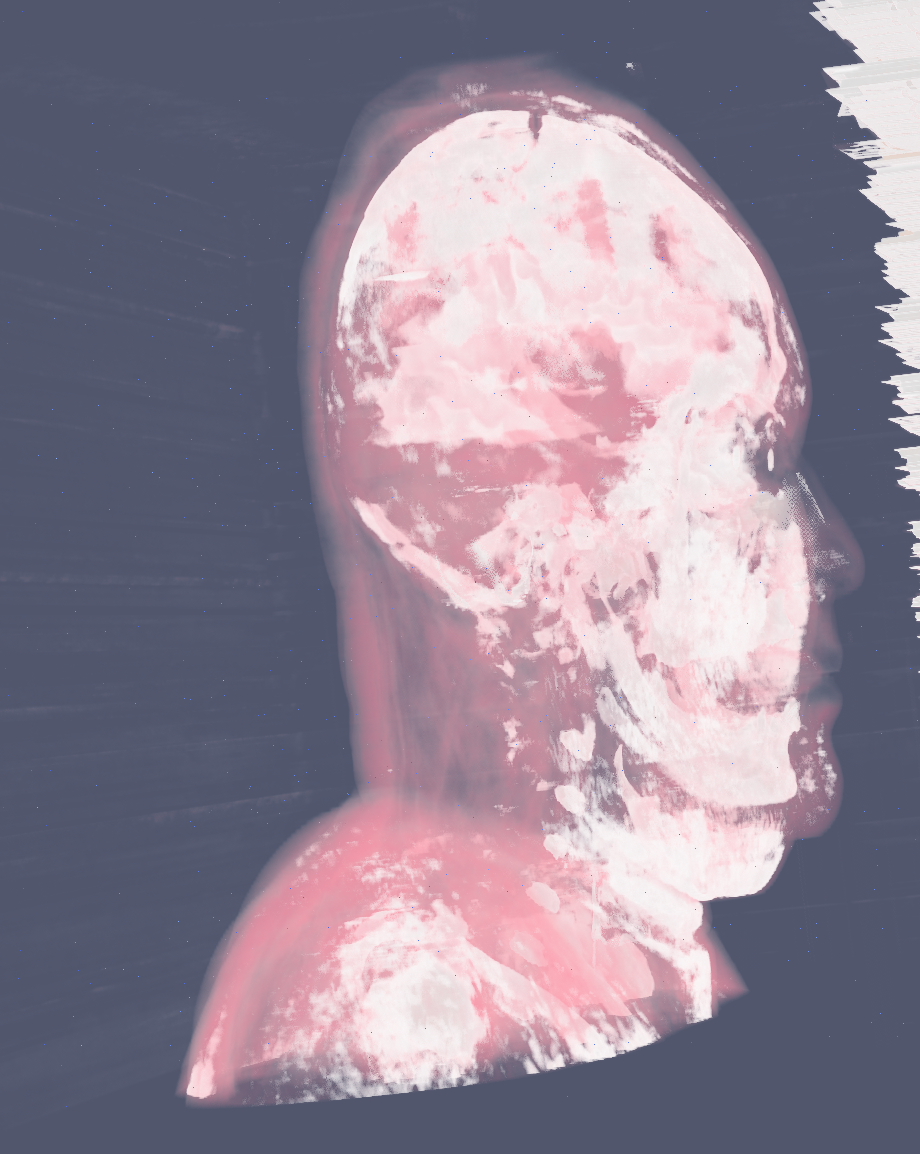
\includegraphics[width=10cm]{Head1.png}
	
	\item[Tool:]
	\hfill \break
		Paraview
	\item[Visual Mappings:]
	
	\begin{itemize}
		\tightlist
		\item[ ]
	\end{itemize}
	
	\begin{itemize}
		\tightlist
		\item
		\textbf{Mapping 1}: 
		\hfill \break
			Pink colour has been assigned to the skin, at data point 157.199 and opacity of 0.013, and white colour has been assigned to the bones, at data point 188.639 with an opacity of 0.562.
	\end{itemize}
	
	\begin{itemize}
		\tightlist
		\item
		\textbf{Mapping 2}:
		\hfill \break
			Colour preset was originally cool to warm but has been modified. Colour space diverging has been used with nan opacity to 1. 
	\end{itemize}
	
	\item[Data Conversion:] 
	\hfill \break
		Data spacing used is 1, 1, 4 with a representation of volume has been used. The volume rendering is using OSPRay based with a blend mode of Composite.
	
	\item[Unique Observation:]
	\hfill \break
		This scan shows a person's head. At data point 188.639 is where the visualisation holds the information for the bones, showing white, and at data point 157.199, is where the skin of the person is. So this shows how the person's bones look under their skin. There is a lightly transparent layer of skin over the top. There seems to be some excess fat in the person's chin.
	
\end{description}
